\section{Разность разностей с контрольными переменными}

\begin{frame}{Линейный пре-тренд: на примере закона в пользу профсоюза учителей\footcite{lovenheim2019long}}

\begin{figure}
    \centering
    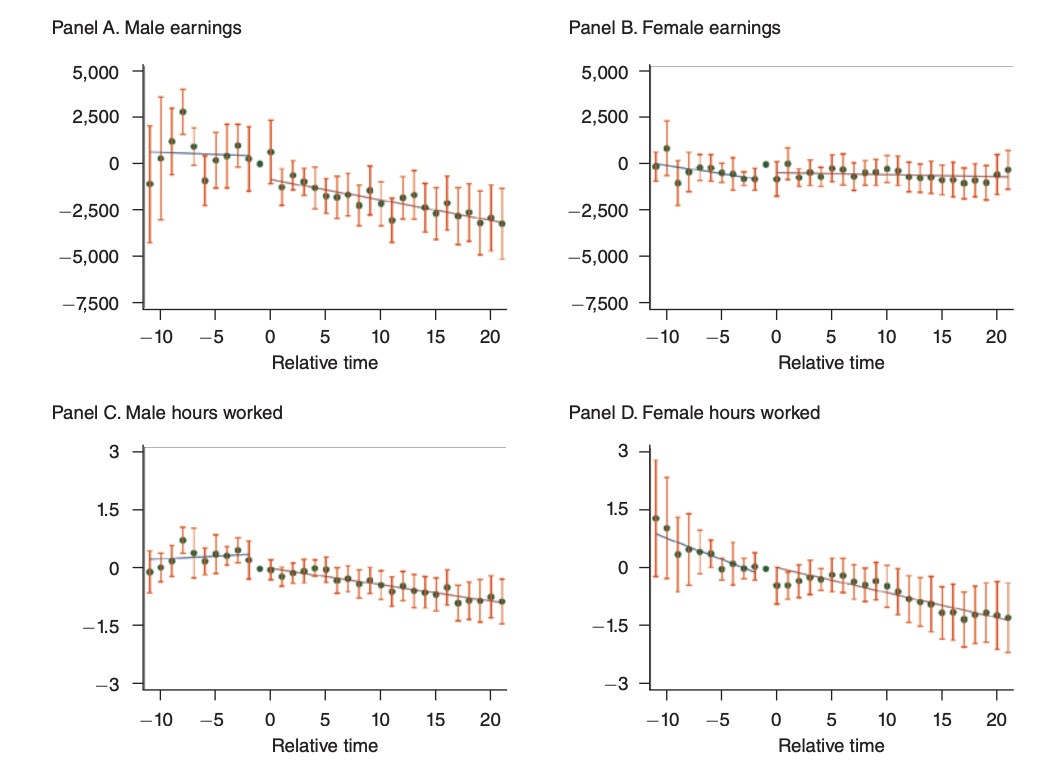
\includegraphics[width=0.8\textwidth]{Images/linear_trends.png}
\end{figure}

\end{frame}
\begin{frame}{Включение линейного тренда}

\begin{align*}
    Y_{it} = & \alpha_0 (t=0) + \alpha_1  (t=1) + \alpha_2 (t=2) + \\
     &+ \tau_0 (t=1) T_{i} + \tau_1 (t=1) T_{i} + \tau_2 (t=2) T_{i} \\
     &+ \beta tT
\end{align*}

\end{frame}

\begin{frame}{Как субсидии помогают покупать качественные продукты?}

\begin{figure}
    \centering
    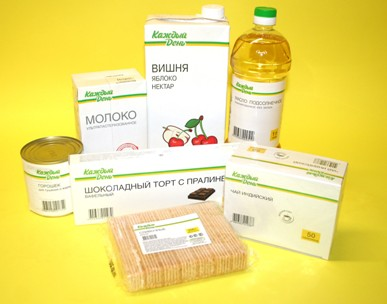
\includegraphics[width=0.7\textwidth]{Images/brand-auchan13.jpg}
    \caption{Store-brand products}
\end{figure}


\end{frame}


\begin{frame}{\textcite{hastings2018snap}}

\begin{figure}
    \centering
    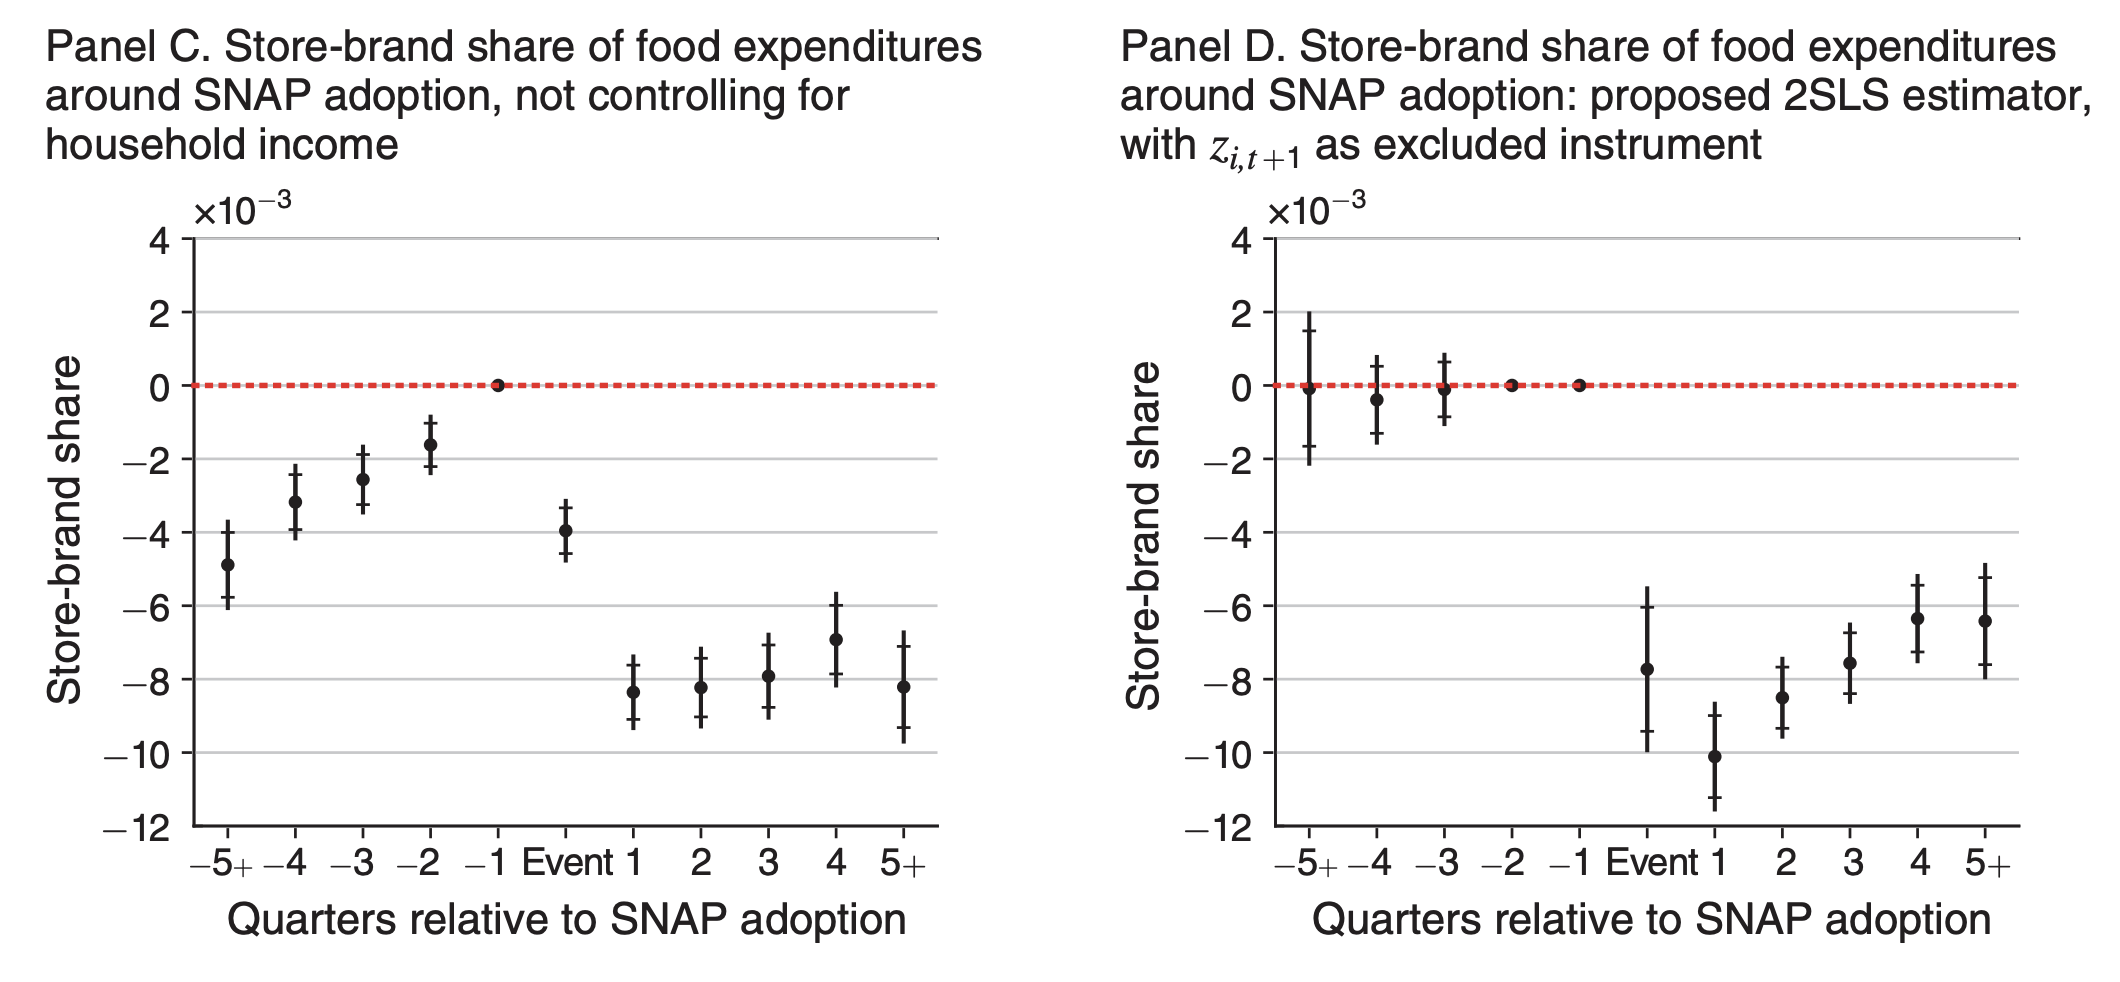
\includegraphics[width=\textwidth]{Images/did_controls.png}
\end{figure}


\end{frame}



\begin{frame}{}

\begin{figure}
    \centering
    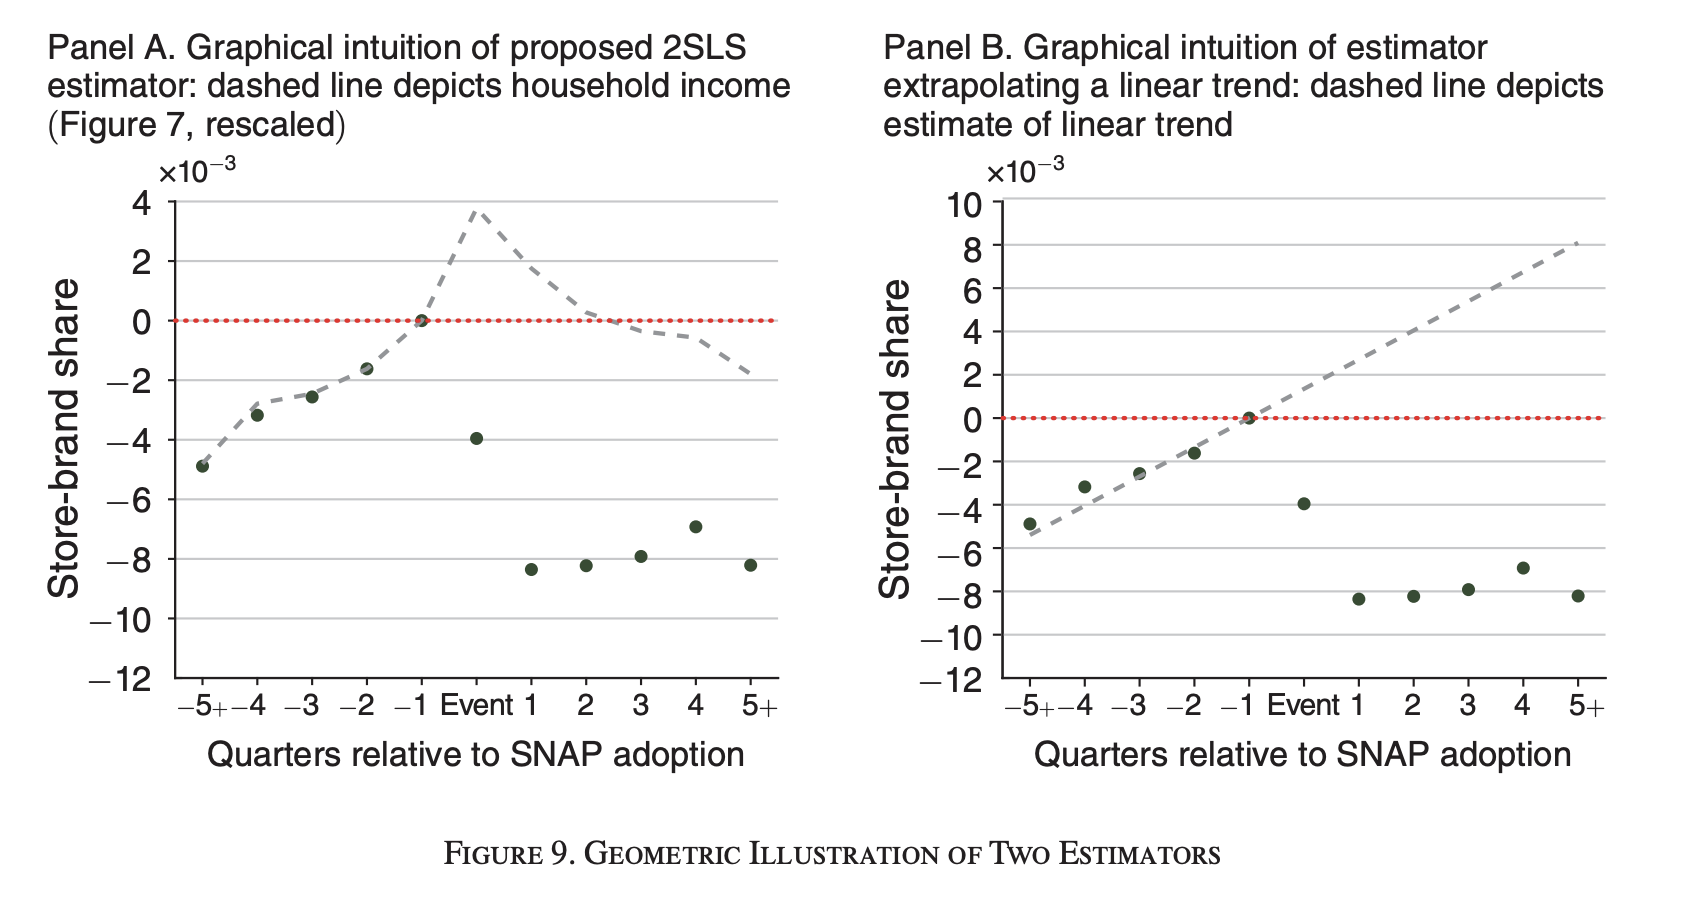
\includegraphics[width=\textwidth]{Images/linear_or_confounder.png}
\end{figure}

\end{frame}

\begin{frame}{Включение контрольных переменных}
Предположим тренды не парралельны, но парралельны условно на X (парралельны для людей с одинаковым уровнем дохода)

\begin{align*}
    Y_{it} = & \alpha_0 (t=0) + \alpha_1  (t=1) + \alpha_2 (t=2) + \\
     &+ \tau_0 (t=1) T_{i} + \tau_1 (t=1) T_{i} + \tau_2 (t=2) T_{i} \\
     &+ X
\end{align*}

% картинку
    
\end{frame}

% \begin{frame}{Что если эффект X меняется во времени?}
% \begin{align*}
% \end{align*}*

% % картинку
    
% \end{frame}

% \begin{frame}{Включение года события}
% \begin{align*}
%     Y_{it} = & \alpha_0 (t=0) + \alpha_1  (t=1) + \alpha_2 (t=2) + \\
%             & \beta_0 (s=0) + \beta_1  (s=1) + \beta_2 (s=2) + \\
%     & \tau_1 (t=1) T_{i} + \tau_2 (t=2) T_{i}
% \end{align*}*

% картинку
    
% \end{frame}

\begin{frame}{Difference-in-Difference-in-Difference}

\begin{figure}
    \centering
    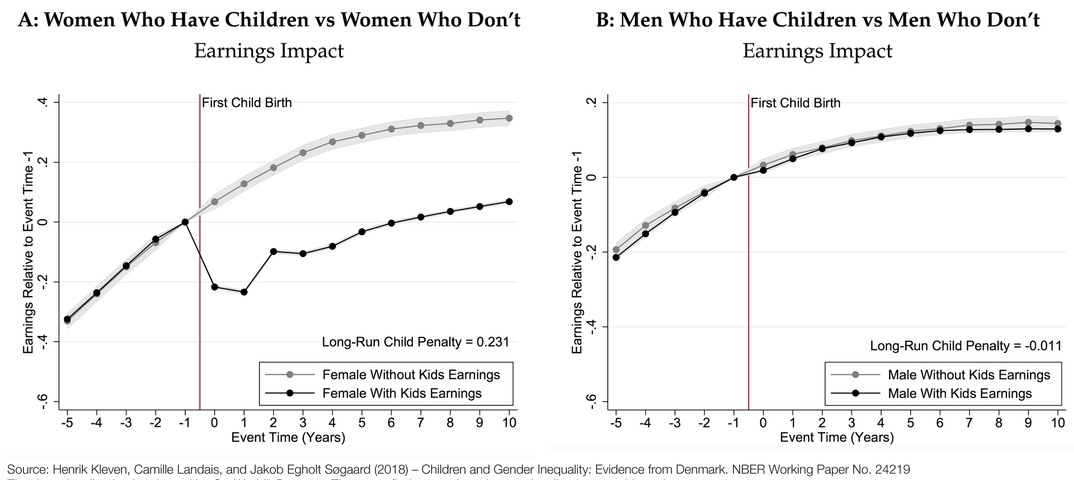
\includegraphics[width=\textwidth]{Images/gender.jpg}
    \label{fig:my_label}
\end{figure}


\end{frame}


% \begin{frame}{Непареметрический контроль (Imbens, Athey)}
% \end{frame}





%%%% APPROXIMATELY CORRECT AND THE IDEA OF MANSKI partial identification approach. 